\documentclass{standalone}
\usepackage{tikz}
\usetikzlibrary{patterns, positioning}

\begin{document}
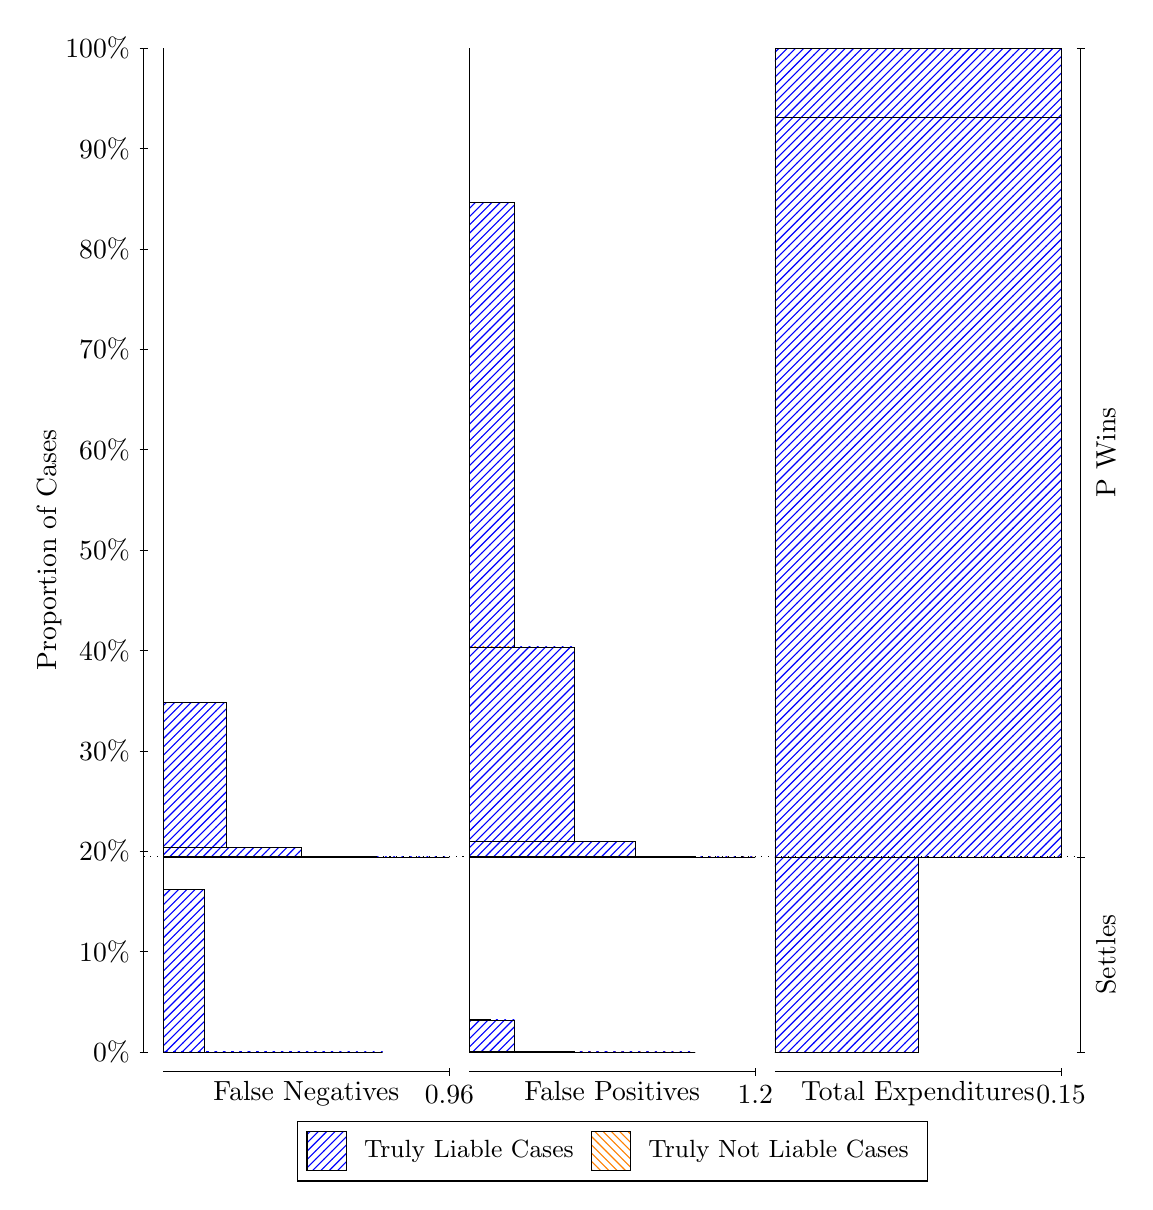
\begin{tikzpicture}
\draw[black, very thin] (1.5,1.75) -- (1.5,14.5);
\node[rotate=90, anchor=center] at (0.3, 8.125) {Proportion of Cases};
\draw[black, very thin] (1.45,1.75) -- (1.55,1.75);
\node[anchor=east] at (1.45, 1.75) {0\%};
\draw[black, very thin] (1.45,3.025) -- (1.55,3.025);
\node[anchor=east] at (1.45, 3.025) {10\%};
\draw[black, very thin] (1.45,4.3) -- (1.55,4.3);
\node[anchor=east] at (1.45, 4.3) {20\%};
\draw[black, very thin] (1.45,5.575) -- (1.55,5.575);
\node[anchor=east] at (1.45, 5.575) {30\%};
\draw[black, very thin] (1.45,6.85) -- (1.55,6.85);
\node[anchor=east] at (1.45, 6.85) {40\%};
\draw[black, very thin] (1.45,8.125) -- (1.55,8.125);
\node[anchor=east] at (1.45, 8.125) {50\%};
\draw[black, very thin] (1.45,9.4) -- (1.55,9.4);
\node[anchor=east] at (1.45, 9.4) {60\%};
\draw[black, very thin] (1.45,10.675) -- (1.55,10.675);
\node[anchor=east] at (1.45, 10.675) {70\%};
\draw[black, very thin] (1.45,11.95) -- (1.55,11.95);
\node[anchor=east] at (1.45, 11.95) {80\%};
\draw[black, very thin] (1.45,13.225) -- (1.55,13.225);
\node[anchor=east] at (1.45, 13.225) {90\%};
\draw[black, very thin] (1.45,14.5) -- (1.55,14.5);
\node[anchor=east] at (1.45, 14.5) {100\%};

\draw[black, very thin] (13.4,1.75) -- (13.4,14.5);
\draw[black, very thin] (13.35,1.75) -- (13.45,1.75);
\node[anchor=west] at (13.35, 1.75) {};
\draw[black, very thin] (13.35,4.2283) -- (13.45,4.2283);
\node[anchor=west] at (13.35, 4.2283) {};
\draw[black, very thin] (13.35,14.5) -- (13.45,14.5);
\node[anchor=west] at (13.35, 14.5) {};

\draw[black, very thin, pattern color=blue, pattern=north east lines] (1.75,1.75) rectangle (4.534,1.75);
\draw[black, very thin, pattern color=blue, pattern=north east lines] (1.75,1.75) rectangle (4.1565,1.75);
\draw[black, very thin, pattern color=blue, pattern=north east lines] (1.75,1.75) rectangle (3.779,1.75);
\draw[black, very thin, pattern color=blue, pattern=north east lines] (1.75,1.75) rectangle (3.5903,1.75);
\draw[black, very thin, pattern color=blue, pattern=north east lines] (1.75,1.75) rectangle (3.4015,1.75);
\draw[black, very thin, pattern color=blue, pattern=north east lines] (1.75,1.75) rectangle (3.2128,1.75);
\draw[black, very thin, pattern color=blue, pattern=north east lines] (1.75,1.75) rectangle (3.024,1.75);
\draw[black, very thin, pattern color=blue, pattern=north east lines] (1.75,1.75) rectangle (2.8353,1.75);
\draw[black, very thin, pattern color=blue, pattern=north east lines] (1.75,1.75) rectangle (2.6465,1.7501);
\draw[black, very thin, pattern color=blue, pattern=north east lines] (1.75,1.7501) rectangle (2.6465,1.7501);
\draw[black, very thin, pattern color=blue, pattern=north east lines] (1.75,1.7501) rectangle (2.4578,1.7501);
\draw[black, very thin, pattern color=blue, pattern=north east lines] (1.75,1.7501) rectangle (2.269,3.8192);
\draw[black, very thin, pattern color=blue, pattern=north east lines] (1.75,3.8192) rectangle (2.0803,3.8192);
\draw[black, very thin, pattern color=blue, pattern=north east lines] (1.75,3.8192) rectangle (1.8916,3.8192);
\draw[black, very thin, pattern color=orange, pattern=north west lines] (1.75,3.8192) rectangle (1.75,3.8192);
\draw[black, very thin, pattern color=blue, pattern=north east lines] (1.75,3.8192) rectangle (1.75,4.2283);
\draw[black, very thin, pattern color=blue, pattern=north east lines] (1.75,4.2283) rectangle (5.3833,4.2283);
\draw[black, very thin, pattern color=blue, pattern=north east lines] (1.75,4.2283) rectangle (4.4396,4.2295);
\draw[black, very thin, pattern color=blue, pattern=north east lines] (1.75,4.2295) rectangle (3.4959,4.3498);
\draw[black, very thin, pattern color=blue, pattern=north east lines] (1.75,4.3498) rectangle (2.5522,6.187);
\draw[black, very thin, pattern color=orange, pattern=north west lines] (1.75,6.187) rectangle (1.75,6.187);
\draw[black, very thin, pattern color=blue, pattern=north east lines] (1.75,6.187) rectangle (1.75,14.5);
\draw[black, very thin, pattern color=orange, pattern=north west lines] (5.6333,1.75) rectangle (8.5018,1.75);
\draw[black, very thin, pattern color=blue, pattern=north east lines] (5.6333,1.75) rectangle (8.5018,1.75);
\draw[black, very thin, pattern color=orange, pattern=north west lines] (5.6333,1.75) rectangle (8.1958,1.75);
\draw[black, very thin, pattern color=blue, pattern=north east lines] (5.6333,1.75) rectangle (8.1958,1.75);
\draw[black, very thin, pattern color=orange, pattern=north west lines] (5.6333,1.75) rectangle (7.8898,1.75);
\draw[black, very thin, pattern color=blue, pattern=north east lines] (5.6333,1.75) rectangle (7.8898,1.75);
\draw[black, very thin, pattern color=blue, pattern=north east lines] (5.6333,1.75) rectangle (7.7368,1.75);
\draw[black, very thin, pattern color=orange, pattern=north west lines] (5.6333,1.75) rectangle (7.5839,1.75);
\draw[black, very thin, pattern color=blue, pattern=north east lines] (5.6333,1.75) rectangle (7.5839,1.75);
\draw[black, very thin, pattern color=blue, pattern=north east lines] (5.6333,1.75) rectangle (7.4309,1.75);
\draw[black, very thin, pattern color=orange, pattern=north west lines] (5.6333,1.75) rectangle (7.2779,1.75);
\draw[black, very thin, pattern color=blue, pattern=north east lines] (5.6333,1.75) rectangle (7.2779,1.75);
\draw[black, very thin, pattern color=blue, pattern=north east lines] (5.6333,1.75) rectangle (7.1249,1.75);
\draw[black, very thin, pattern color=orange, pattern=north west lines] (5.6333,1.75) rectangle (6.9719,1.75);
\draw[black, very thin, pattern color=blue, pattern=north east lines] (5.6333,1.75) rectangle (6.9719,1.7535);
\draw[black, very thin, pattern color=blue, pattern=north east lines] (5.6333,1.7535) rectangle (6.8189,1.7535);
\draw[black, very thin, pattern color=blue, pattern=north east lines] (5.6333,1.7535) rectangle (6.666,1.7535);
\draw[black, very thin, pattern color=orange, pattern=north west lines] (5.6333,1.7535) rectangle (6.666,1.7535);
\draw[black, very thin, pattern color=blue, pattern=north east lines] (5.6333,1.7535) rectangle (6.666,1.7546);
\draw[black, very thin, pattern color=blue, pattern=north east lines] (5.6333,1.7546) rectangle (6.513,1.7547);
\draw[black, very thin, pattern color=blue, pattern=north east lines] (5.6333,1.7547) rectangle (6.36,1.7547);
\draw[black, very thin, pattern color=blue, pattern=north east lines] (5.6333,1.7547) rectangle (6.207,2.1564);
\draw[black, very thin, pattern color=blue, pattern=north east lines] (5.6333,2.1564) rectangle (6.054,2.1564);
\draw[black, very thin, pattern color=blue, pattern=north east lines] (5.6333,2.1564) rectangle (5.9011,2.1564);
\draw[black, very thin, pattern color=blue, pattern=north east lines] (5.6333,2.1564) rectangle (5.9011,2.1591);
\draw[black, very thin, pattern color=blue, pattern=north east lines] (5.6333,2.1591) rectangle (5.7481,2.1591);
\draw[black, very thin, pattern color=blue, pattern=north east lines] (5.6333,2.1591) rectangle (5.6333,4.2283);
\draw[black, very thin, pattern color=orange, pattern=north west lines] (5.6333,4.2283) rectangle (9.2667,4.2283);
\draw[black, very thin, pattern color=blue, pattern=north east lines] (5.6333,4.2283) rectangle (9.2667,4.2283);
\draw[black, very thin, pattern color=orange, pattern=north west lines] (5.6333,4.2283) rectangle (8.5018,4.2283);
\draw[black, very thin, pattern color=blue, pattern=north east lines] (5.6333,4.2283) rectangle (8.5018,4.2309);
\draw[black, very thin, pattern color=orange, pattern=north west lines] (5.6333,4.2309) rectangle (7.7368,4.2309);
\draw[black, very thin, pattern color=blue, pattern=north east lines] (5.6333,4.2309) rectangle (7.7368,4.4221);
\draw[black, very thin, pattern color=orange, pattern=north west lines] (5.6333,4.4221) rectangle (6.9719,4.4221);
\draw[black, very thin, pattern color=blue, pattern=north east lines] (5.6333,4.4221) rectangle (6.9719,6.8949);
\draw[black, very thin, pattern color=orange, pattern=north west lines] (5.6333,6.8949) rectangle (6.207,6.8949);
\draw[black, very thin, pattern color=blue, pattern=north east lines] (5.6333,6.8949) rectangle (6.207,12.541);
\draw[black, very thin, pattern color=blue, pattern=north east lines] (5.6333,12.541) rectangle (5.6333,14.5);
\draw[black, very thin, pattern color=orange, pattern=north west lines] (9.5167,1.75) rectangle (11.333,1.75);
\draw[black, very thin, pattern color=blue, pattern=north east lines] (9.5167,1.75) rectangle (11.333,4.2283);
\draw[black, very thin, pattern color=orange, pattern=north west lines] (9.5167,4.2283) rectangle (13.15,4.2283);
\draw[black, very thin, pattern color=blue, pattern=north east lines] (9.5167,4.2283) rectangle (13.15,13.619);
\draw[black, very thin, pattern color=orange, pattern=north west lines] (9.5167,13.619) rectangle (13.15,13.619);
\draw[black, very thin, pattern color=blue, pattern=north east lines] (9.5167,13.619) rectangle (13.15,14.5);
\draw[black, dotted] (1.5,4.2283) -- (13.4,4.2283);
\draw[black, very thin] (1.75,1.5) -- (5.3833,1.5);
\node[anchor=north] at (3.5667, 1.5) {False Negatives};
\draw[black, very thin] (5.3833,1.45) -- (5.3833,1.55);
\node[anchor=north] at (5.3833, 1.45) {0.96};

\draw[black, very thin] (5.6333,1.5) -- (9.2667,1.5);
\node[anchor=north] at (7.45, 1.5) {False Positives};
\draw[black, very thin] (9.2667,1.45) -- (9.2667,1.55);
\node[anchor=north] at (9.2667, 1.45) {1.2};

\draw[black, very thin] (9.5167,1.5) -- (13.15,1.5);
\node[anchor=north] at (11.333, 1.5) {Total Expenditures};
\draw[black, very thin] (13.15,1.45) -- (13.15,1.55);
\node[anchor=north] at (13.15, 1.45) {0.15};

\node[black, centered, rotate=90] at (13.72, 2.9892) {Settles};
\node[black, centered, rotate=90] at (13.72, 9.3642) {P Wins};

\draw (7.449999999999999,1.5) node[draw=none] (baseCoordinate) {};
\begin{scope}[align=center]
        \matrix[scale=0.5, draw=black, below=0.5cm of baseCoordinate, nodes={draw}, column sep=0.1cm]{
            \node[rectangle, draw, minimum width=0.5cm, minimum height=0.5cm, pattern=north east lines, pattern color=blue] {}; &
            \node[draw=none, font=\small] (B) {Truly Liable Cases}; &
            \node[rectangle, draw, minimum width=0.5cm, minimum height=0.5cm, pattern=north west lines, pattern color=orange] {}; &
            \node[draw=none, font=\small] (B) {Truly Not Liable Cases}; \\
            };
\end{scope}

\end{tikzpicture}
\end{document}